\documentclass[aspectratio=169]{beamer}

\usepackage{amsmath,amssymb}
\usepackage{booktabs}
\usepackage{tabularx}
\usepackage{colortbl}
\usepackage{multimedia}
\usepackage{tikz}
\usetikzlibrary{arrows.meta,backgrounds,calc,positioning,shapes.multipart,fit}
\usepackage[main=english]{babel}
\usepackage{ragged2e}

\definecolor{fortranPurple}{HTML}{503874}  % poster deep purple
\definecolor{fortranPurpleMid}{HTML}{7E5AA6}
\usetheme[
  accent=fortranPurple,
  progressbar=foot,
  sectionpage=progressbar,
  subsectionpage=progressbar,
  numbering=fraction,
  numberrail=section,
  block=fill,
  notes=hide,
  toc=aftertitle,
  closing=contact
]{cookie}


% complexity badge helper
\newcommand{\cplx}[1]{{\footnotesize\color{cookieMuted}#1}}
\newcommand{\muted}[1]{{\footnotesize\color{cookieMuted}#1}}

% Widen the footer author box so the three institutions fit (default is .18\paperwidth)
\makeatletter
\setbeamertemplate{footline}{%
  \leavevmode\vbox{%
    \ifdefstring{\cookie@progressbar}{foot}{\hbox{\cookie@progressrule{\paperwidth}}}{}%
    \hbox{%
      \begin{beamercolorbox}[wd=.36\paperwidth,ht=2.7ex,dp=1.15ex,leftskip=.02\paperwidth]{footline}%
        \usebeamerfont{footline}\insertshortauthor
      \end{beamercolorbox}%
      \begin{beamercolorbox}[wd=.46\paperwidth,ht=2.7ex,dp=1.15ex,leftskip=.012\paperwidth,rightskip=.012\paperwidth]{footline}%
        \usebeamerfont{footline}\insertshorttitle%
        \ifx\insertsectionhead\@empty\else\hfill\cookie@footersection{\insertsectionhead}\fi%
      \end{beamercolorbox}%
      \begin{beamercolorbox}[wd=.18\paperwidth,ht=2.7ex,dp=1.15ex,leftskip=.027\paperwidth,rightskip=.014\paperwidth plus 1fil]{footline right}%
        \usebeamerfont{footline number}\strut\cookie@insertnumber
      \end{beamercolorbox}%
    }%
  }%
}

\title[1 m$^2$ ANUGA]{Seventeen billion triangles}
\subtitle{A 1\,m$^2$ flood model of the Mahanadi delta, tiled onto GPUs}
\author[NCI]{Jorge Luis G\'alvez Vallejo \textnormal{(NCI)}}
\cookieemail{jorge.galvezvallejo@anu.edu.au}
\institute{NCI}
\cookieuni{Australian National University}
\cookielocation{Canberra, Australia}
\date{\today}
\cookietagline{GPU porting \& optimization at NCI}
%\cookietitleimage{assets/cookie-background.png}

\titlegraphic{%
  \begin{tabular}{@{}c@{}}
    \begin{tcolorbox}[enhanced,colback=white,colframe=white,boxrule=0pt,
        arc=5pt,width=3.1cm,left=7pt,right=7pt,top=8pt,bottom=8pt,
        halign=center,valign=center,nobeforeafter,box align=center]
      
\includegraphics[height=1.05cm]{assets/nci.png}\\[.8em]
      % PLACEHOLDER: second logo -- drop the real file in as assets/logo2.png
      
\includegraphics[height=1.05cm]{assets/logo2.png}
    \end{tcolorbox}%
  \end{tabular}%
}
\cookieclosingtitle{Thank you}
\cookieclosingtext{Tiles in, water out.}
\cookieclosingqr{https://github.com/anuga-community/anuga_core}
\cookieclosingqrlabel{ANUGA}


\begin{document}

\maketitle

% =====================================================================
\section{Problem}

\begin{frame}{Problem}{11,372 km$^2$ of delta at 1\,m$^2$}
  \begin{columns}[T,onlytextwidth]
    \column{.52\textwidth}
      \begin{itemize}\setlength\itemsep{5pt}
        \item \textbf{17.45 billion triangles}
        \item ANUGA \texttt{Domain} in Python: $\sim$1\,KB per triangle $\Rightarrow$ 17\,TB
        \item A merged mesh: $\sim$1\,TB of connectivity; no partitioner can hold it
        \item Device memory: 512\,B per triangle $\Rightarrow$ 8.9\,TB $\Rightarrow$ at least 62 H200s
      \end{itemize}
    \column{.44\textwidth}
      \begin{block}{So}
        \begin{itemize}
          \item Never build the global mesh, elevation, or output
          \item Read tiles straight into the GPU domain, in C
        \end{itemize}
      \end{block}
  \end{columns}
\end{frame}

% =====================================================================
\section{Tiling}

\begin{frame}{Tiling}{Cutting the polygon so tiles can be meshed independently}
  \begin{columns}[T,onlytextwidth]
    \column{.5\textwidth}
      \begin{enumerate}\setlength\itemsep{4pt}
        \item Densify the delta outline to a fixed spacing $s$ \muted{($s = 1.2$\,m at 1\,m$^2$, just under the natural edge length)}
        \item Intersect with a regular grid of 3\,km cells \muted{(64 $\times$ 46, 1404 non-empty)}
        \item Every cut line is rebuilt from \textbf{lattice points}: origin $+\,k\,s$ along the line, from one common origin
        \item Tag segments: \texttt{exterior} (outline) or \texttt{internal} (cut)
      \end{enumerate}
    \column{.46\textwidth}
      \begin{block}{Why it conforms}
        Both tiles sharing a cut line reproduce the same lattice points, because the lattice depends only on the global origin and $s$ --- not on the tile.
      \end{block}
      \begin{block}{Meshing}
        Triangle with \texttt{-Y}: no vertices inserted on segments, so a tile's edge is exactly its lattice points. One process per tile: 1404 tiles in 26 min on 104 cores.
      \end{block}
  \end{columns}
\end{frame}

\begin{frame}{Tiling}{Two adjacent 1\,m$^2$ tiles, triangulated independently}
  \centering
  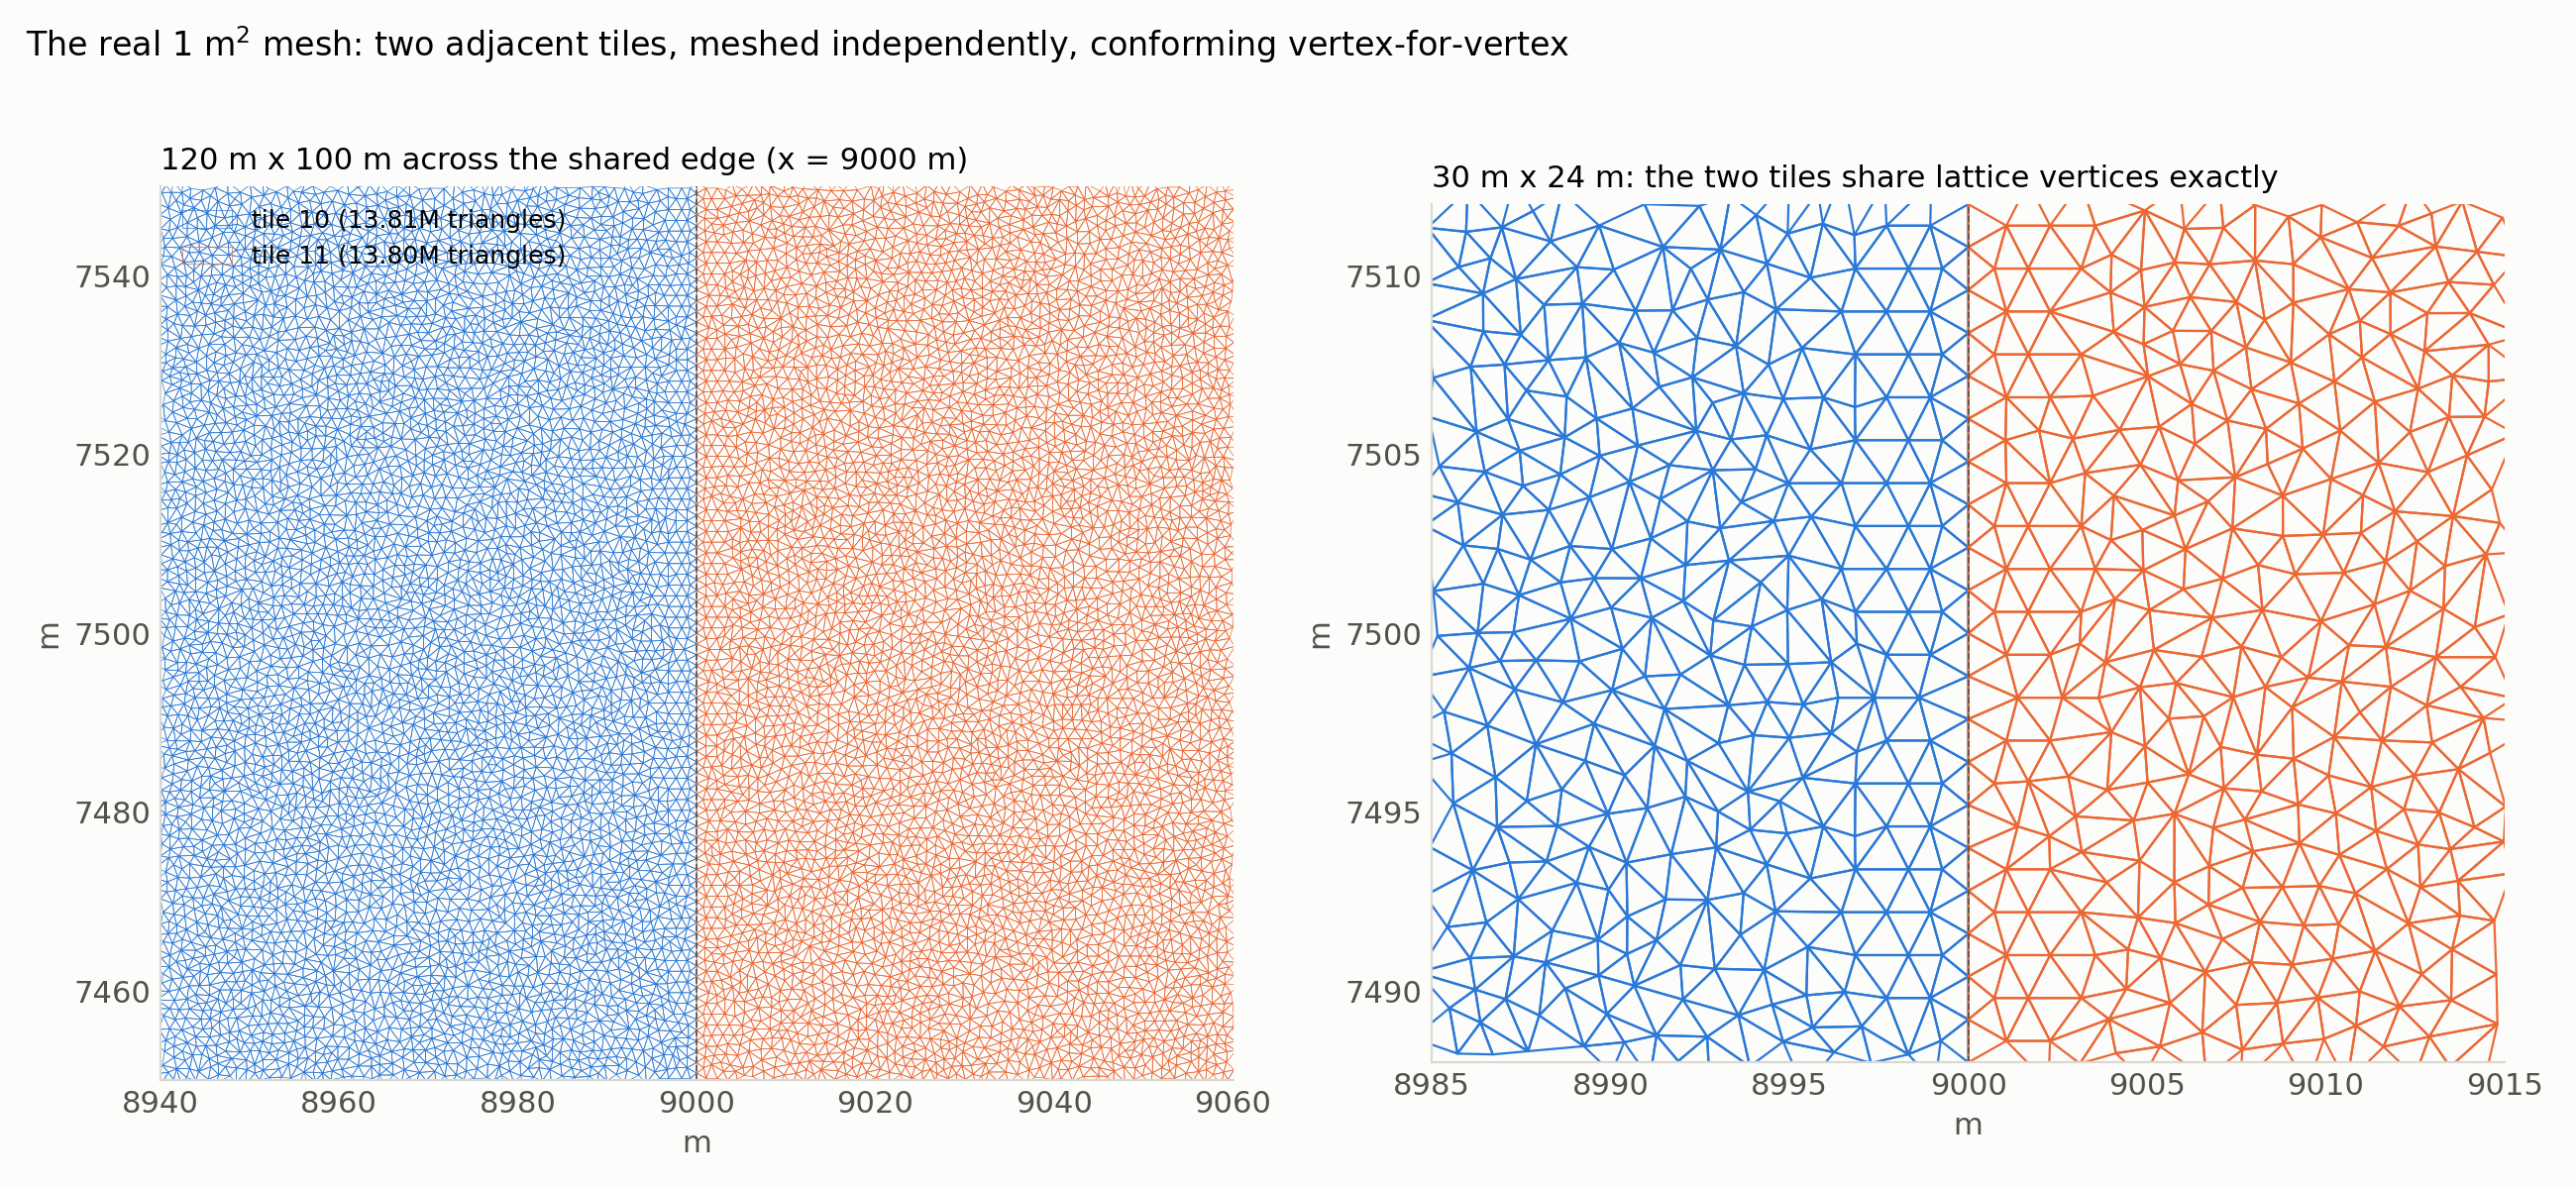
\includegraphics[width=.98\textwidth,height=.78\textheight,keepaspectratio]{figs/fig8_mesh_zoom.png}
\end{frame}

\begin{frame}{Refining}{Splitting a tile without touching its neighbours}
  \begin{columns}[T,onlytextwidth]
    \column{.5\textwidth}
      \begin{itemize}\setlength\itemsep{5pt}
        \item A flagged tile becomes four half-size sub-tiles; the new cut lines carry the same global lattice
        \item The sub-tile corner lands in the middle of a neighbour's edge --- it conforms only if that midpoint is a lattice point: \textbf{half-tile must be a multiple of $s$} \muted{(1500\,m / 1.2\,m = 1250)}
        \item Only the sub-tiles are re-meshed; every other tile's mesh is reused
        \item 13 tiles $\to$ 50 sub-tiles in minutes
      \end{itemize}
    \column{.46\textwidth}
      \begin{block}{Stitching}
        Vertices are rounded to 6 decimals identically everywhere, then merged on exact equality. Neighbours across a cut are found by matching edge keys --- the same rule whether one process merges all tiles or each rank stitches its own.
      \end{block}
  \end{columns}
\end{frame}

\begin{frame}{Scales}{Not every tile needs 1\,m$^2$}
  \begin{columns}[T,onlytextwidth]
    \column{.5\textwidth}
      \begin{itemize}\setlength\itemsep{4pt}
        \item Each tile gets its own maximum area from a map (the coarse run's wetness); areas nest as $A \cdot 4^k$ so lattice spacings nest as $s \cdot 2^k$
        \item A shared cut line carries the \textbf{finer} lattice --- both tiles compute the same points, so they still conform; Triangle grades into the coarse side
        \item Delta test: 1024 / 256 / 64\,m$^2$ $\Rightarrow$ 20M triangles instead of 355M uniform; bit-exact tiled vs merged
        \item Ganges-scale: 2\,M\,km$^2$ is $\sim$3\,T triangles at 1\,m$^2$; with 5\,\% at 1\,m$^2$, 25\,\% at 25, the rest coarse: $\sim$185\,G
      \end{itemize}
      \muted{Time step: set by triangles at outline/cut-line corners, not by the transitions --- keeping lattice points half a spacing from corners gave 1.38$\times$ on $\Delta t$.}
    \column{.48\textwidth}
      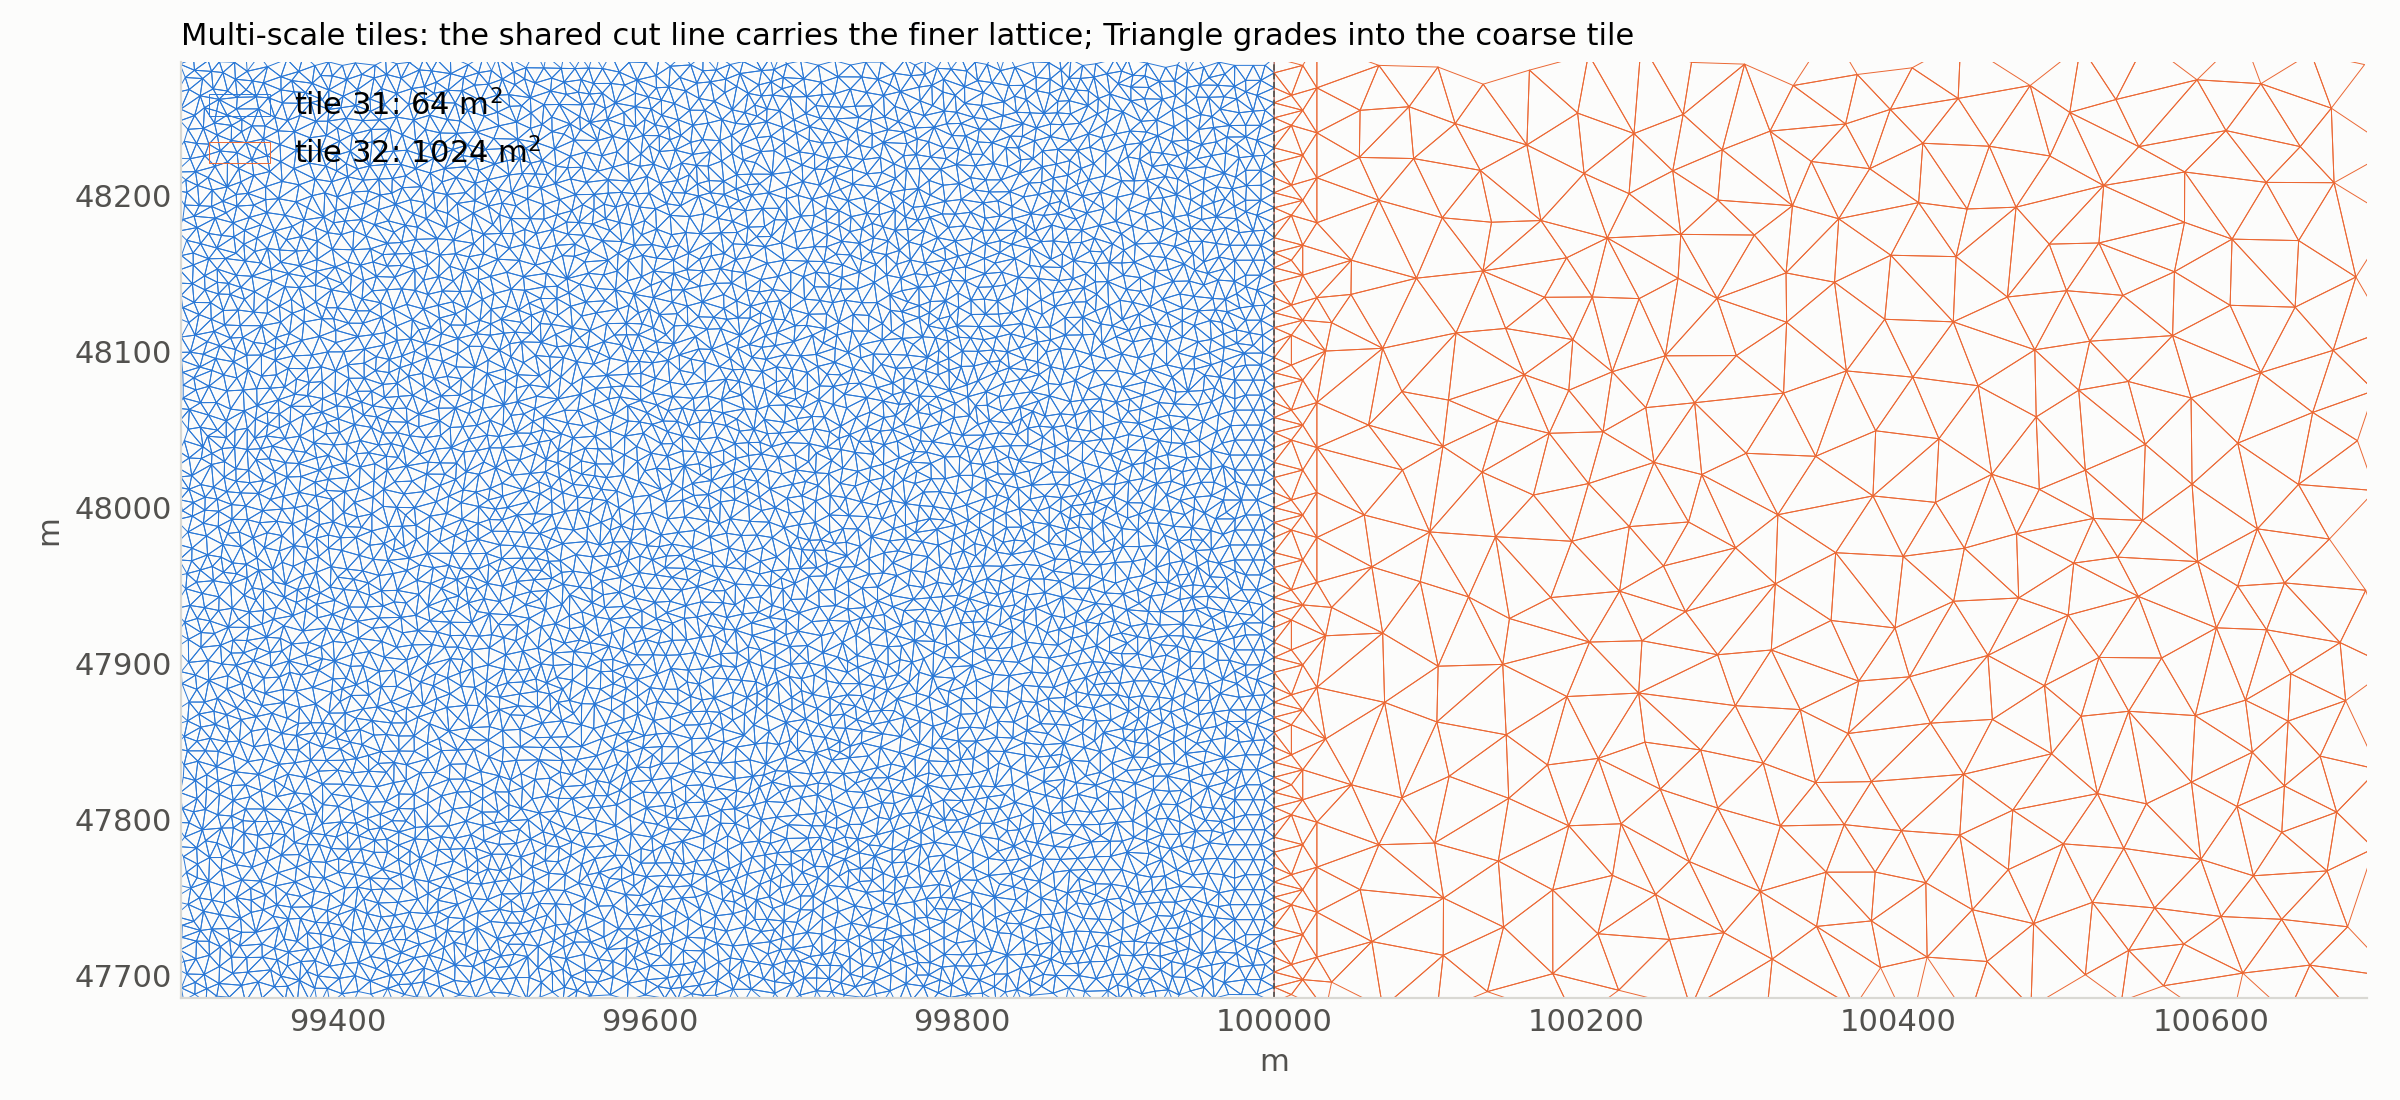
\includegraphics[width=\textwidth]{figs/fig9_multiscale_transition.png}
  \end{columns}
\end{frame}

\begin{frame}{Corners}{Where the time step is set}
  \begin{columns}[T,onlytextwidth]
    \column{.44\textwidth}
      \begin{itemize}\setlength\itemsep{4pt}
        \item ANUGA's $\Delta t = \min(\text{inradius} / \text{speed})$ over wet cells: the smallest triangle on the wet edge decides everything
        \item The smallest triangles were not in the resolution transitions --- they were at \textbf{outline / cut-line corners}: intersection points millimetres from an outline vertex, and lattice points a few metres from a corner, which Triangle's 28$^\circ$ rule fills with slivers
        \item Rule: no inserted point within $0.5\,s$ of a segment endpoint, no outline vertex within $s$ of a corner's cut line --- symmetric on both sides, so tiles still conform
        \item Same mesh: $\Delta t$ 0.032 $\to$ 0.045\,s (1.38$\times$); the lake now has one triangle below half the median inradius out of 3.25\,M
      \end{itemize}
    \column{.54\textwidth}
      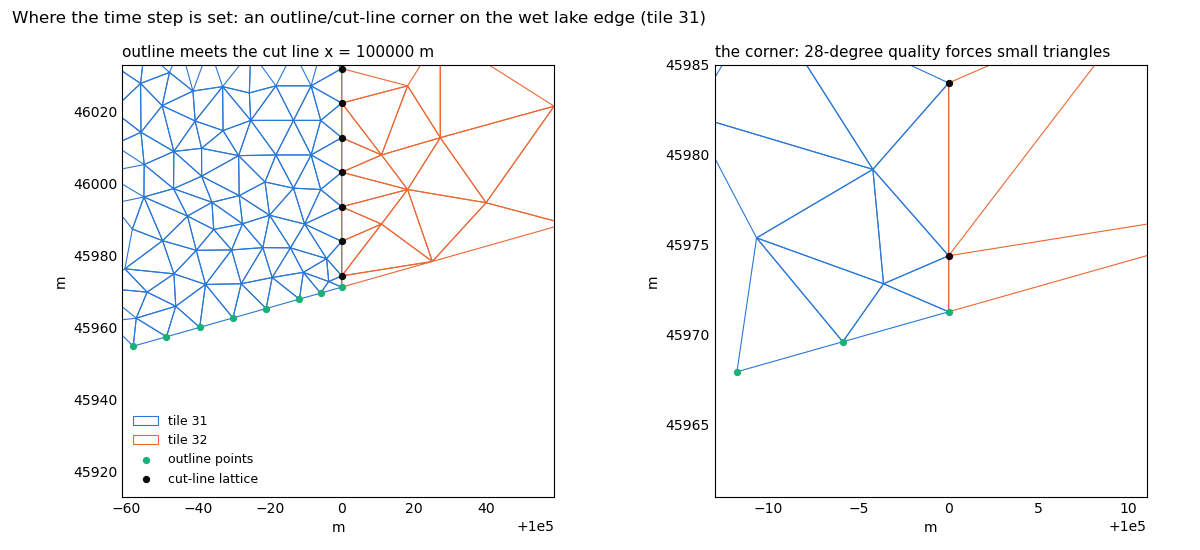
\includegraphics[width=\textwidth]{figs/fig11_corner.png}
  \end{columns}
\end{frame}

\begin{frame}{Tiles}{1441 tiles after refinement; the rehearsal block near the synthetic lake}
  \centering
  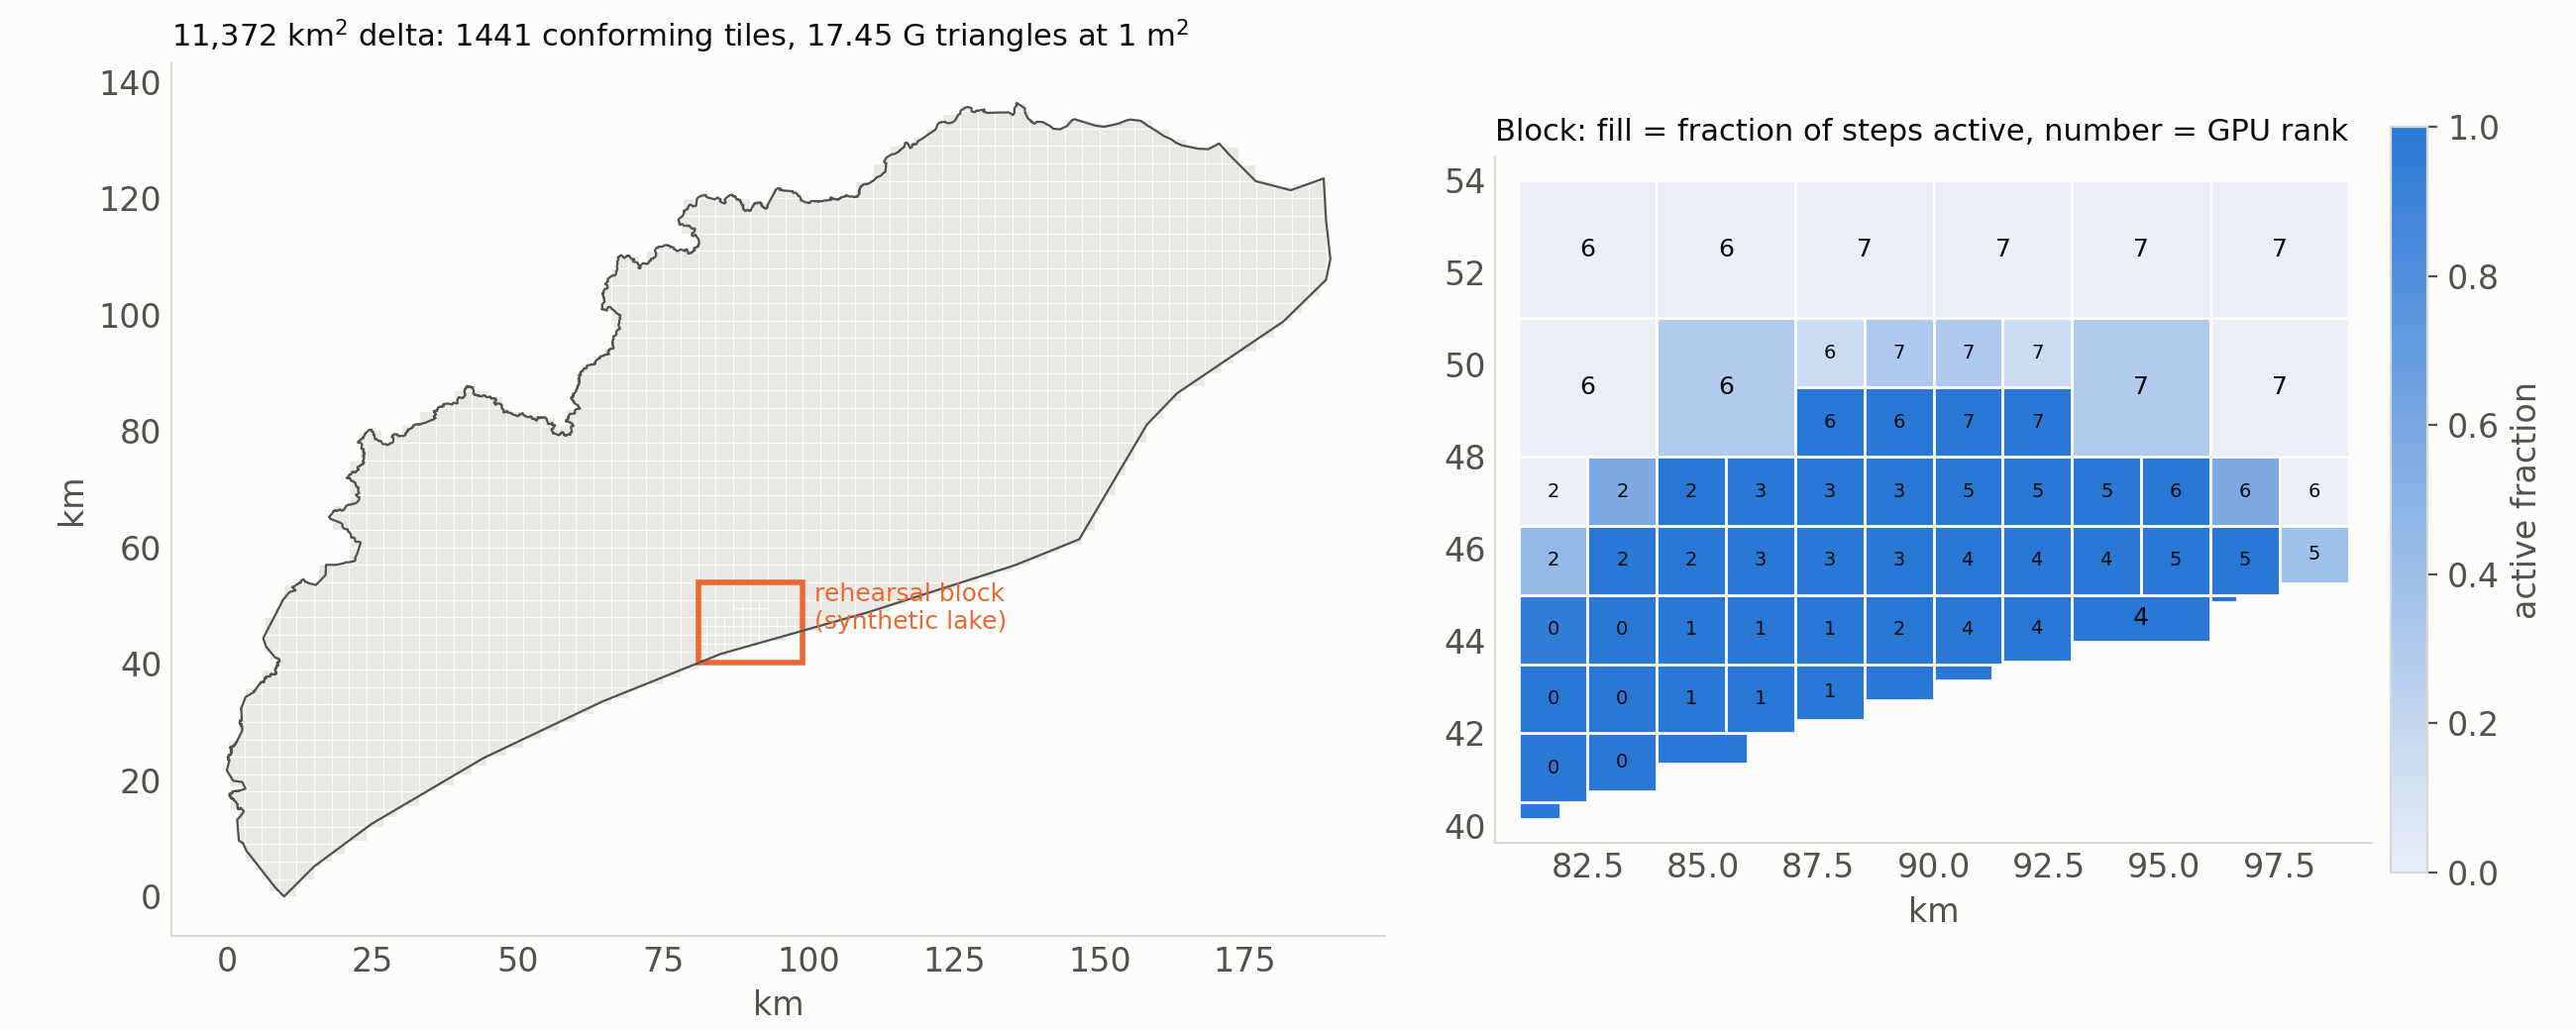
\includegraphics[width=.98\textwidth,height=.78\textheight,keepaspectratio]{figs/fig5_tile_map.png}
\end{frame}

% =====================================================================
\section{Launching}

\begin{frame}{Pipeline}{Every stage is tile-parallel}
  \centering
  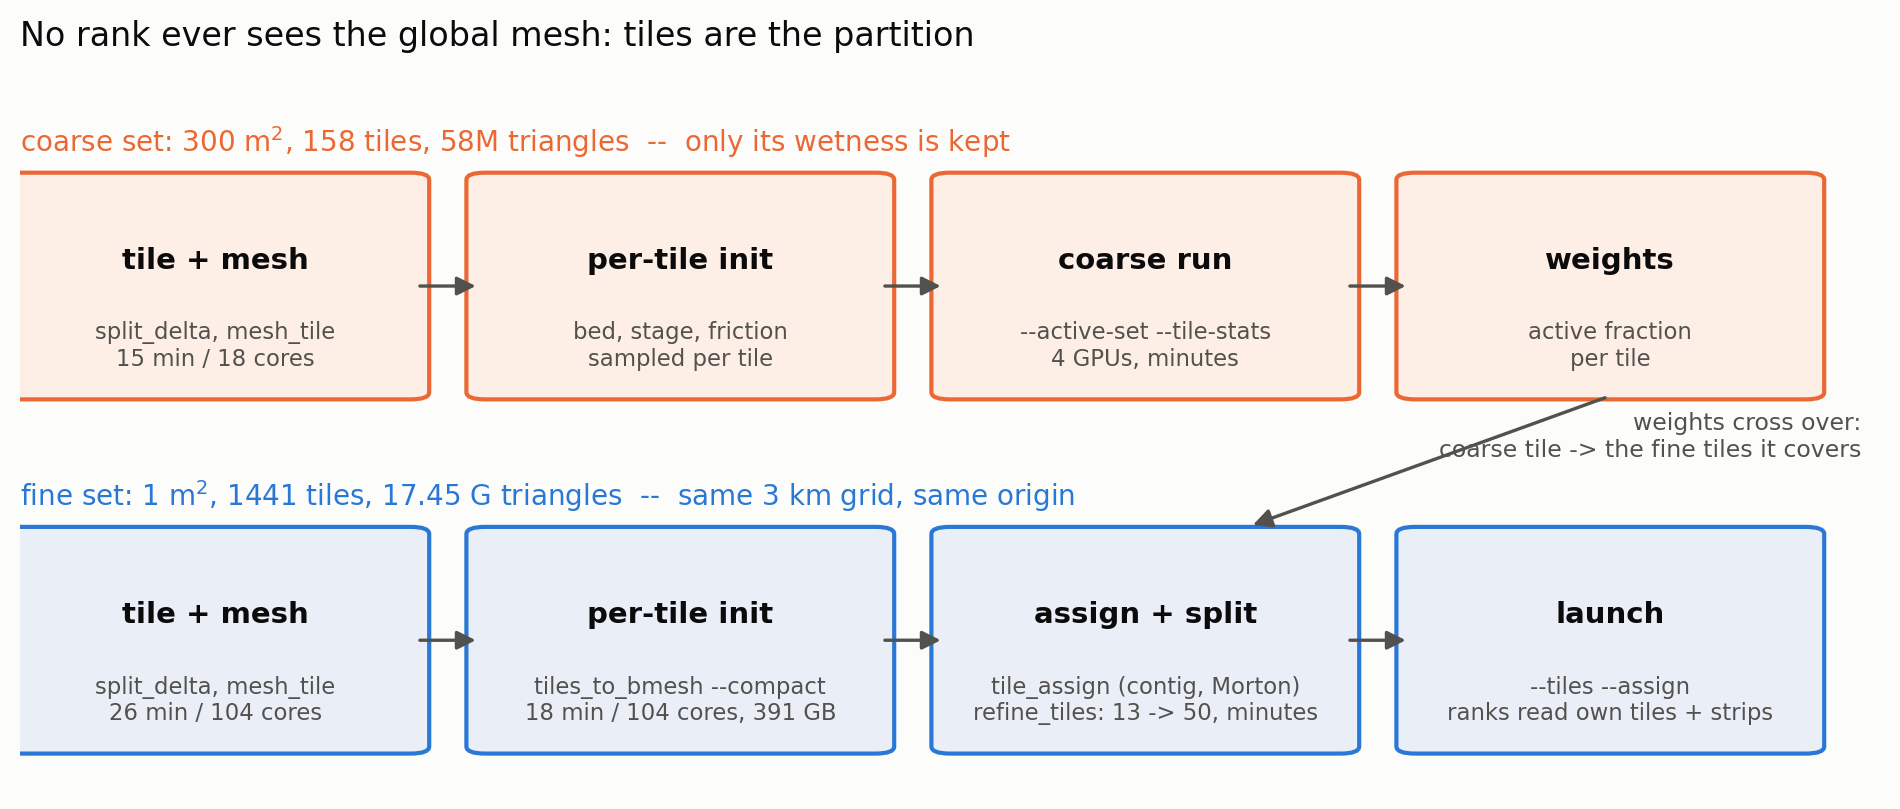
\includegraphics[width=.98\textwidth,height=.72\textheight,keepaspectratio]{figs/fig7_pipeline.png}
\end{frame}

\begin{frame}{Launching}{\texttt{--tiles index.txt --assign ranks.txt}}
  \begin{columns}[T,onlytextwidth]
    \column{.52\textwidth}
      \begin{enumerate}\setlength\itemsep{4pt}
        \item A rank reads its tiles plus every tile whose bounding box touches them
        \item Stitches on exact vertex coordinates
        \item Ghosts: foreign triangles sharing a vertex with an owned one \muted{(covers the 2-hop ring RK2 needs)}
        \item Halo lists derived on both sides from the same data, in the same order --- nothing to negotiate
      \end{enumerate}
    \column{.44\textwidth}
      \begin{block}{Checked}
        \begin{itemize}
          \item Tiled vs merged mesh: bit-exact, np = 1, 2, 4, 7
          \item Real 1\,m$^2$ tiles: np = 8 over two nodes bit-exact vs np = 4
          \item Scatter fluxes: $10^{-15}$ of field scale
        \end{itemize}
      \end{block}
  \end{columns}
\end{frame}

\begin{frame}{Scaling}{C-only MPI across GPUs, slab partition of a generated mesh}
  \centering
  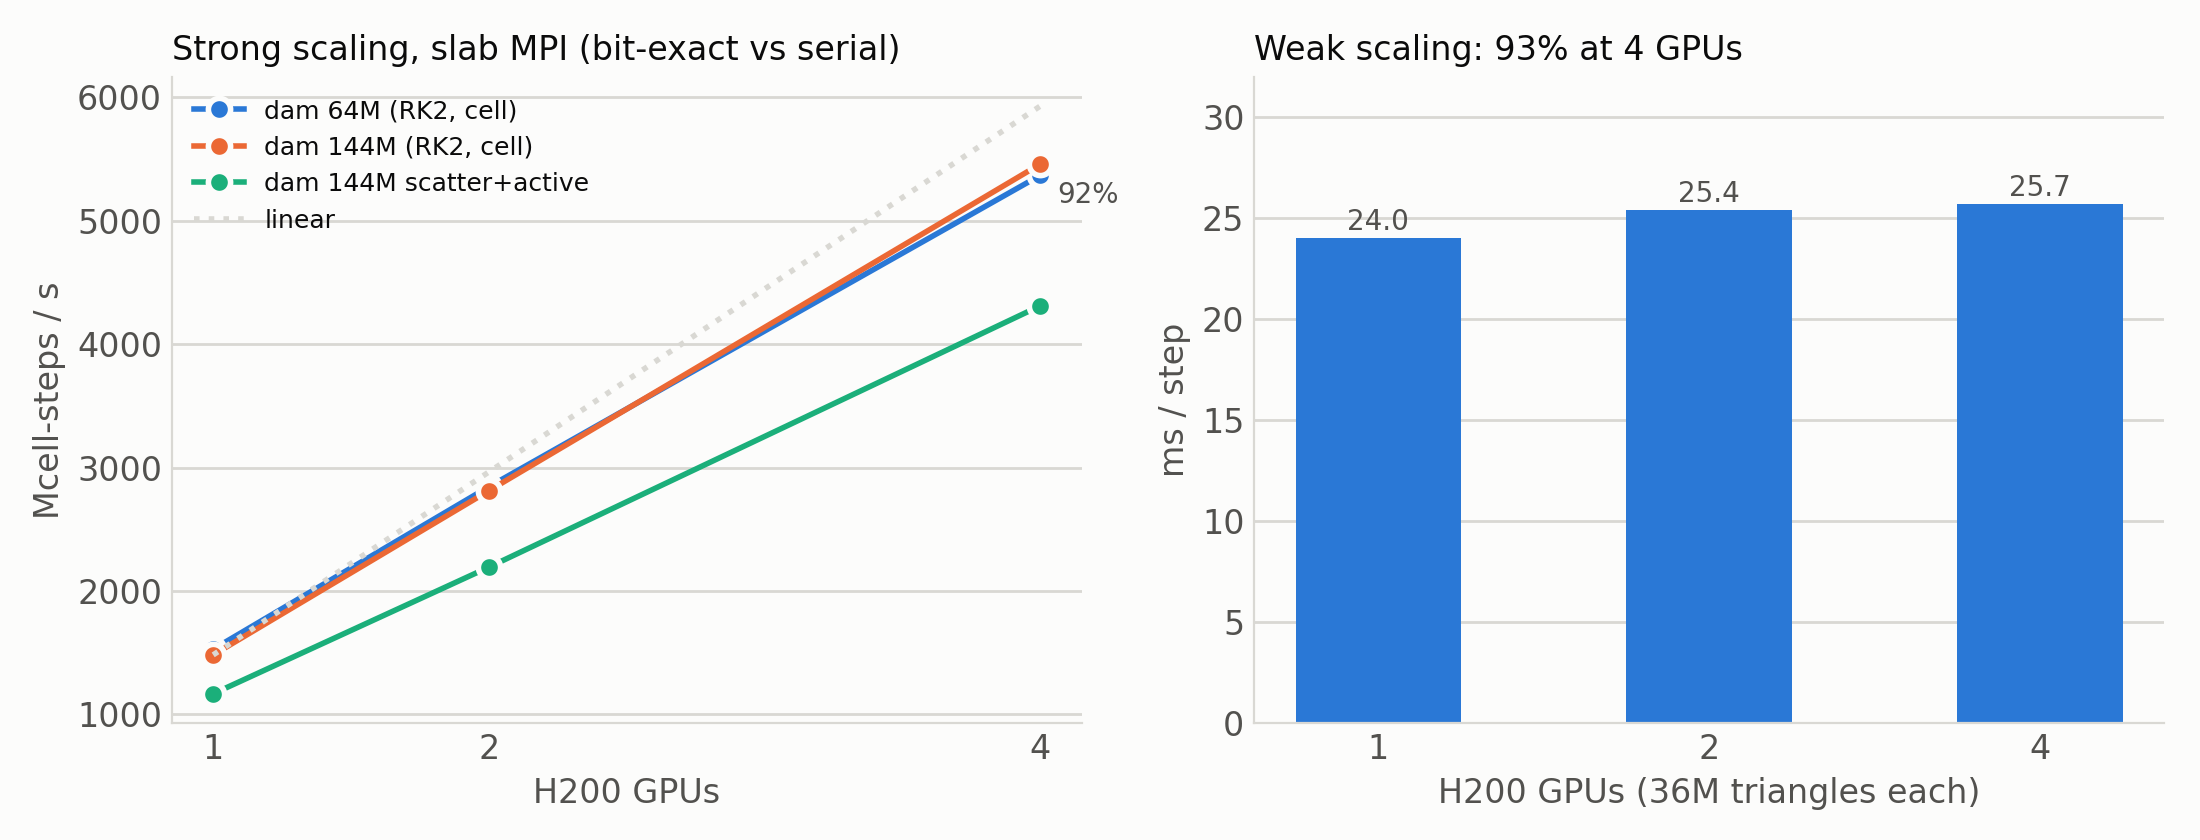
\includegraphics[width=.98\textwidth,height=.74\textheight,keepaspectratio]{figs/fig1_slab_scaling.png}
\end{frame}

\begin{frame}{Portability}{Same C source, unmodified: nvc, amdclang, icx --- digit-identical physics on all five}
  \centering
  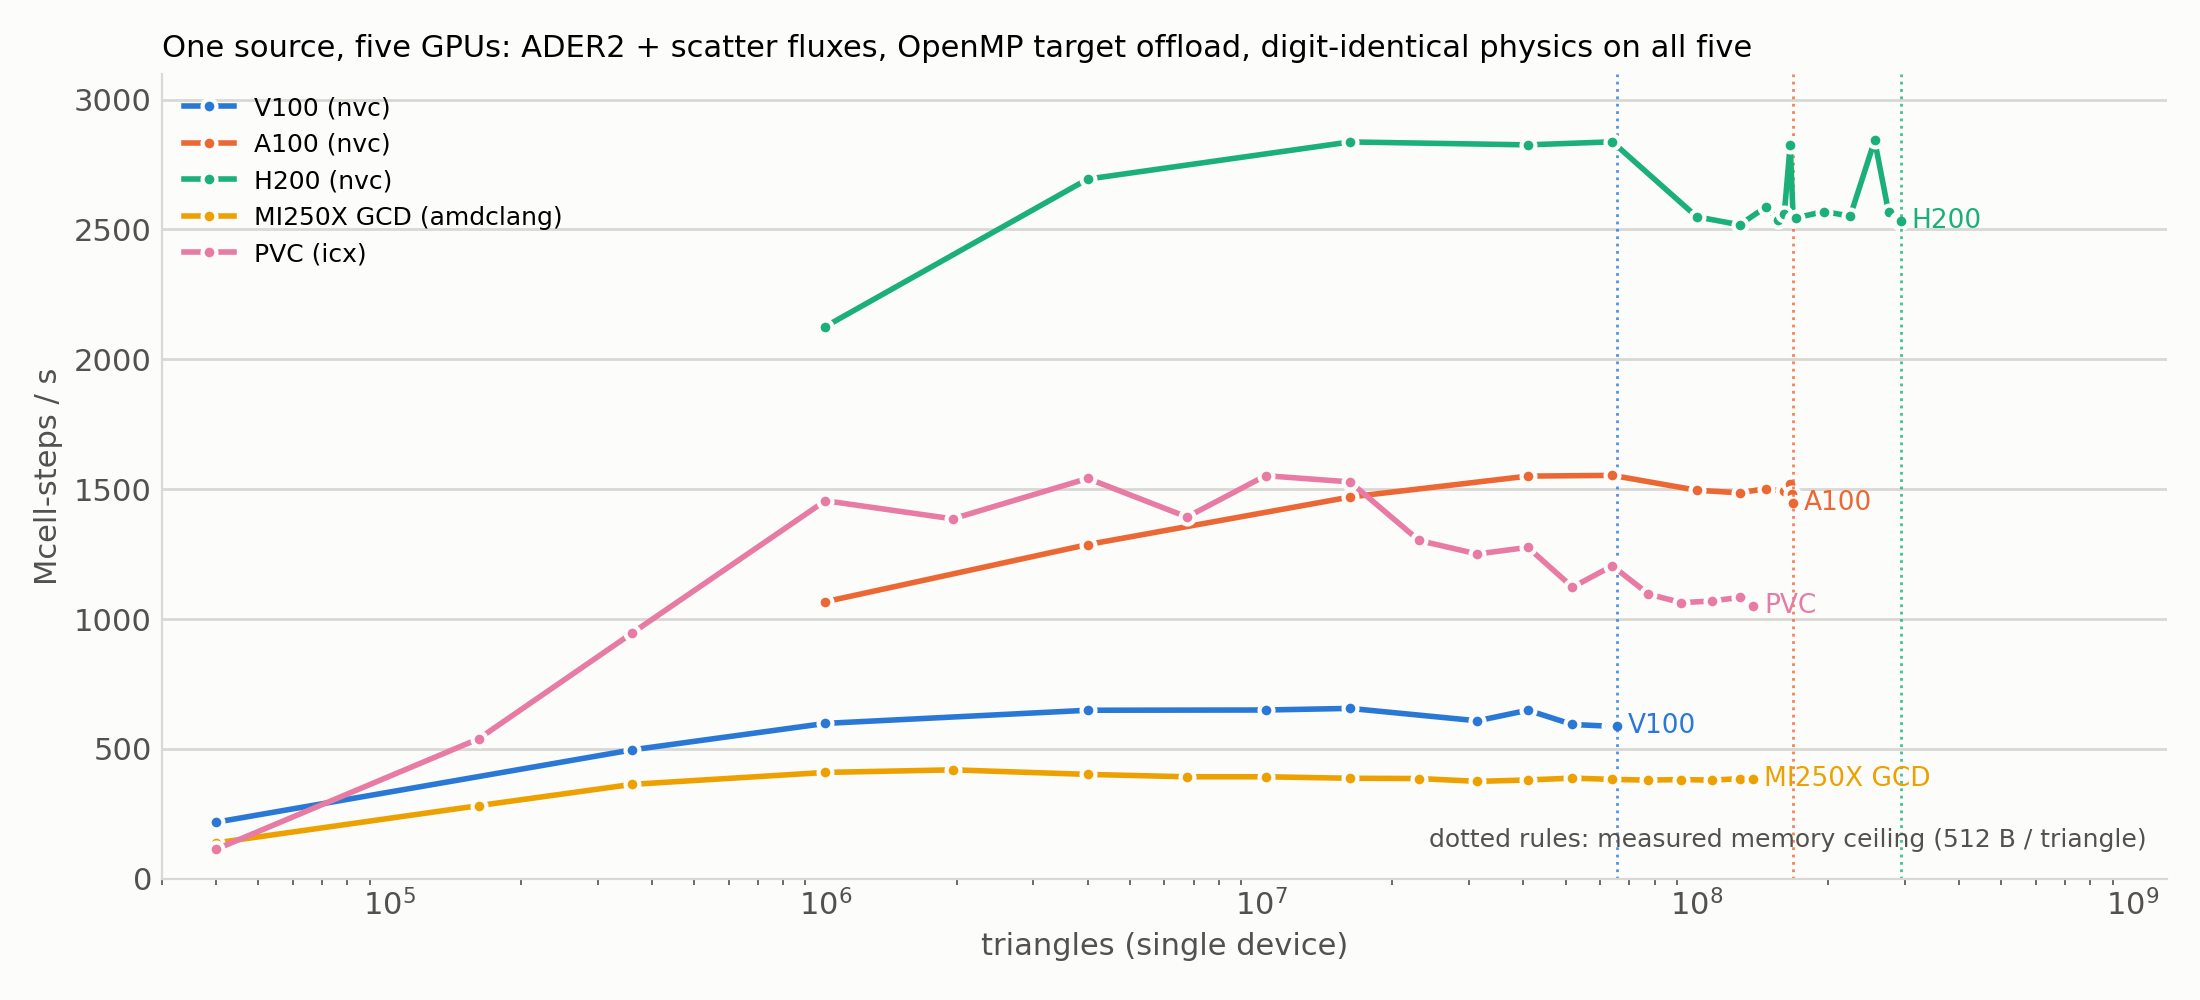
\includegraphics[width=.98\textwidth,height=.76\textheight,keepaspectratio]{figs/fig10_portability.png}
\end{frame}

\begin{frame}{Portability}{Where each device lands, and what the AMD gap is}
  \begin{columns}[T,onlytextwidth]
    \column{.56\textwidth}
      \begin{tabular}{@{}lrrrr@{}}
        \toprule
        device & peak & plateau & HBM & Mc/s per TB/s \\
        \midrule
        V100 16 GB      & 656  & $\sim$650  & 0.9 TB/s & $\sim$720 \\
        A100 80 GB      & 1553 & $\sim$1500 & 2.0 TB/s & $\sim$750 \\
        H200 143 GB     & 2843 & $\sim$2550 & 4.8 TB/s & $\sim$530 \\
        PVC 64 GB       & 1552 & $\sim$1060 & 1.6 TB/s & $\sim$660 \\
        MI250X GCD 64 GB& 419  & $\sim$385  & 1.6 TB/s & \textbf{$\sim$240} \\
        \bottomrule
      \end{tabular}
      \muted{Mcell-steps/s, ADER2 + scatter, single device; plateau = large-mesh value. Volume drift $\le 10^{-16}$, zero NaNs, identical max-momentum on every device at all 19 common sizes.}
    \column{.4\textwidth}
      \begin{block}{Reading it}
        \begin{itemize}
          \item NVIDIA plateaus track bandwidth; the MI250X GCD is the flattest curve measured (no fade to 134.6M)
          \item Per unit of bandwidth CDNA runs at a third of the others: a 2--3$\times$ target, not a tuning one
          \item First suspect: the AMD build has no \texttt{-munsafe-fp-atomics}, so the six fp64 atomic adds per edge in the scatter kernel compile to CAS loops
        \end{itemize}
      \end{block}
  \end{columns}
\end{frame}

% =====================================================================
\section{Balancing}

\begin{frame}{Imbalance}{Most of a basin is dry; the active set makes cost follow the water}
  \centering
  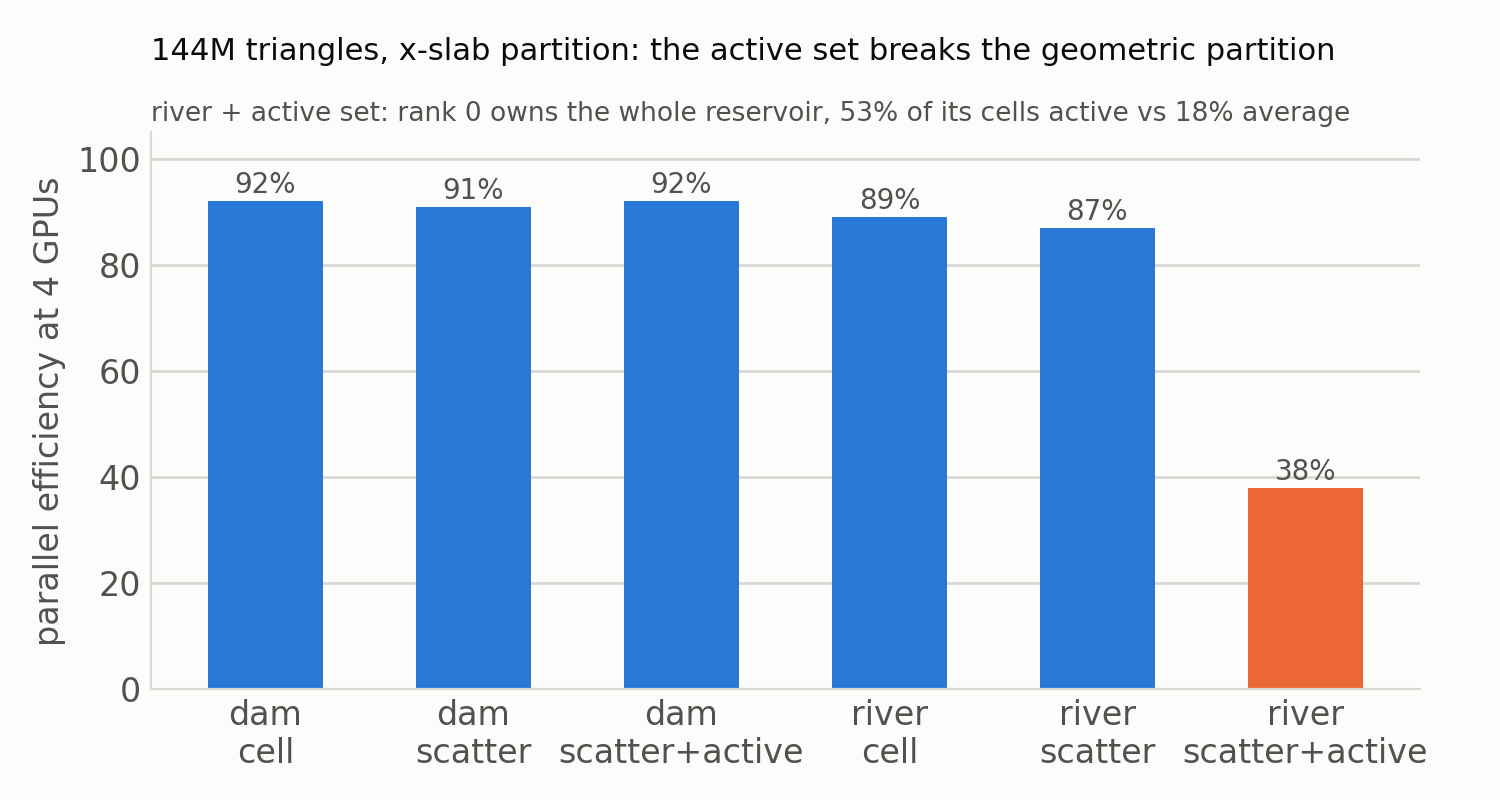
\includegraphics[width=.9\textwidth,height=.74\textheight,keepaspectratio]{figs/fig2_slab_active_imbalance.png}
\end{frame}

\begin{frame}{Weighting}{A cost model measured on the H200}
  \begin{columns}[T,onlytextwidth]
    \column{.46\textwidth}
      \[
        w(\text{tile}) = n_{\text{tri}} \times (\text{active fraction} + 0.073)
      \]
      \begin{itemize}\setlength\itemsep{4pt}
        \item 0.073\,ns per cell of never-skipped work, 1.0\,ns per active cell
        \item Active fraction per tile from a coarse run
        \item Contiguous split in Morton order; split tiles above a quarter of a rank's share
        \item Predicted vs measured active cells per rank: 373k/178k/15k/17k vs 374k/179k/15k/17k
      \end{itemize}
    \column{.52\textwidth}
      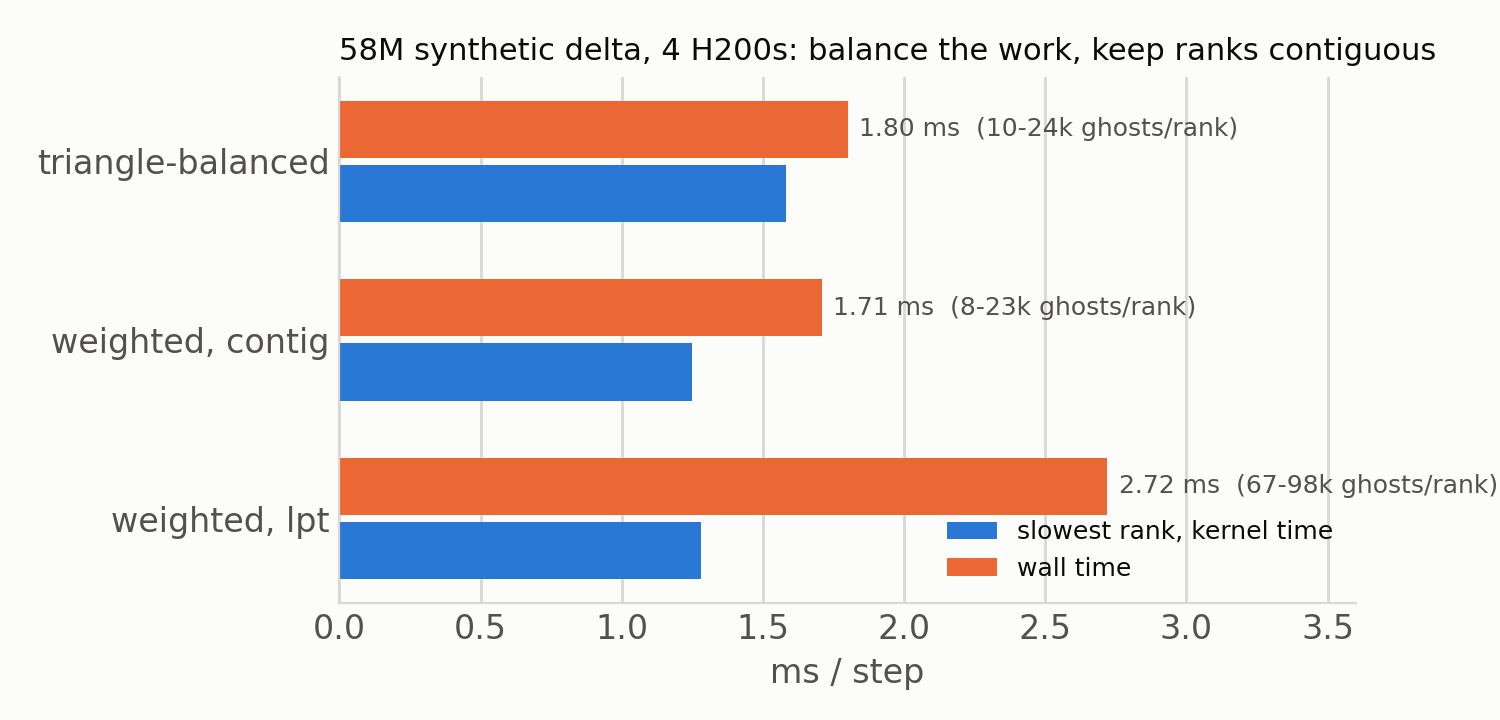
\includegraphics[width=\textwidth]{figs/fig6_300sqm_contig_vs_lpt.png}
  \end{columns}
\end{frame}

\begin{frame}{Balancing}{301M real triangles, 8 H200s on two nodes}
  \centering
  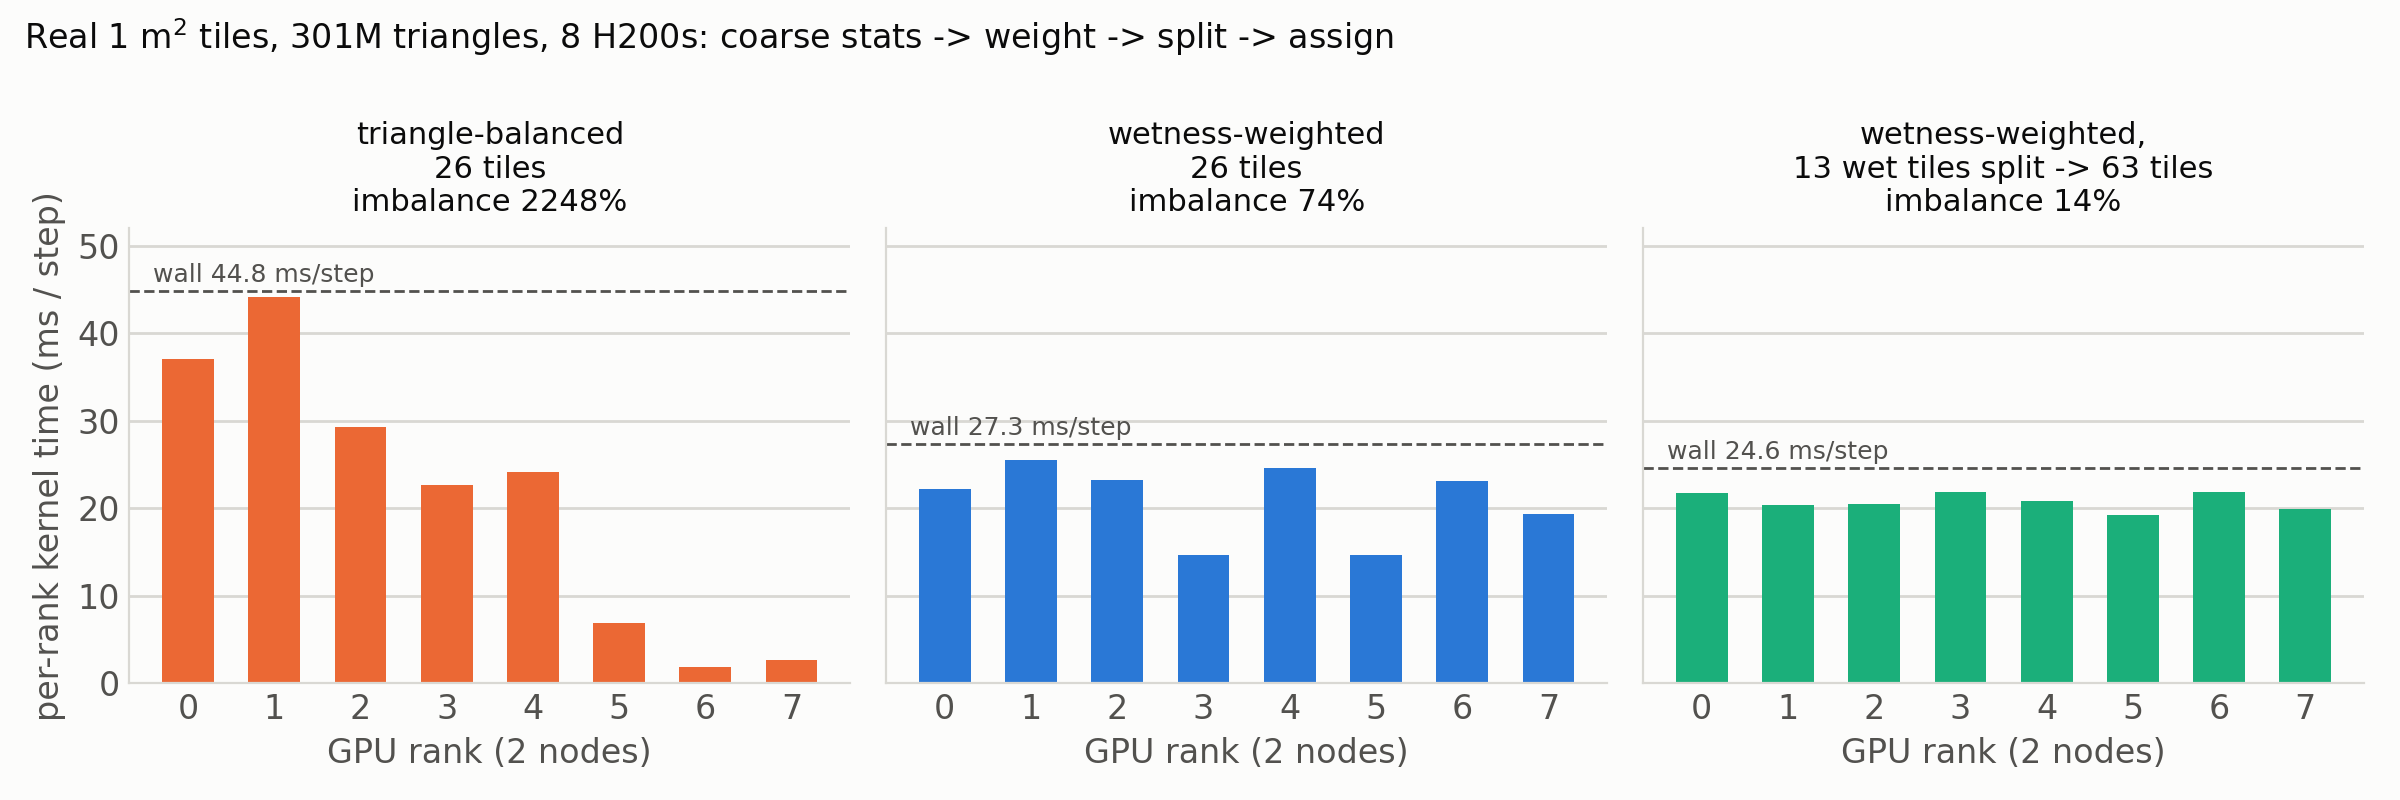
\includegraphics[width=.98\textwidth,height=.76\textheight,keepaspectratio]{figs/fig3_1sqm_balance_ranks.png}
\end{frame}

\begin{frame}{Time}{Same block; every run bit-exact against the np = 4 golden}
  \centering
  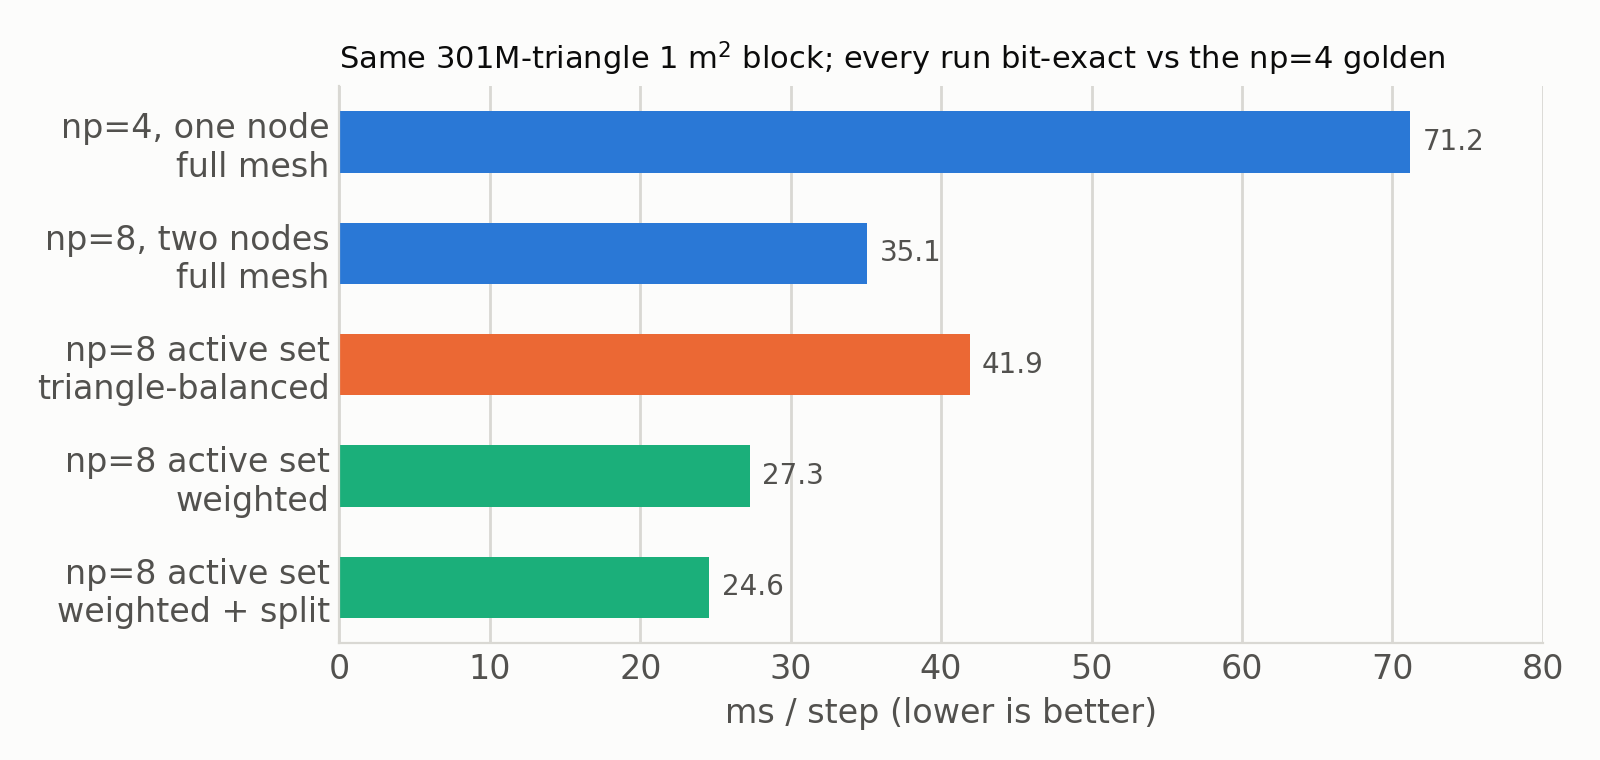
\includegraphics[width=.9\textwidth,height=.74\textheight,keepaspectratio]{figs/fig4_1sqm_walltime.png}
\end{frame}

% =====================================================================
\section{Outlook}

\begin{frame}{Costs}{Measured on real 1\,m$^2$ tiles}
  \begin{columns}[T,onlytextwidth]
    \column{.5\textwidth}
      \begin{block}{Per triangle}
        \begin{itemize}
          \item Device 488\,B, host 543\,B
          \item Build 0.45\,\textmu s \muted{(a 200M-triangle rank: $\sim$90\,s)}
          \item 4 $\to$ 8 GPUs across nodes: 89--100\%
        \end{itemize}
      \end{block}
      \begin{block}{Stages}
        \begin{itemize}
          \item Mesh: 26 min, convert and initialise: 18 min \muted{(104 cores)}
          \item Refine 13 tiles: minutes
        \end{itemize}
      \end{block}
    \column{.46\textwidth}
      \begin{block}{Full mesh, 17.45 G triangles}
        \begin{itemize}
          \item 8.5\,TB device: 62 H200s minimum, $\sim$100 realistic
          \item 9.5\,TB host: 25 gpuhopper nodes
          \item $\Delta t \approx 0.07$\,s: 1.2M steps per simulated day; the active set decides the hours
        \end{itemize}
      \end{block}
  \end{columns}
\end{frame}

\begin{frame}{Data}{Gridded inputs onto 17 billion triangles}
  \begin{columns}[T,onlytextwidth]
    \column{.5\textwidth}
      \begin{block}{Expensive: the fit}
        \texttt{set\_quantity(filename, alpha)} is a least-squares fit with smoothing --- a sparse solve over the mesh. At 8.7\,G vertices it cannot run, and at 1\,m$^2$ it can only blur the 1\,m LiDAR.
      \end{block}
      \begin{block}{Cheap: sampling per tile}
        \begin{itemize}
          \item Elevation: read the raster window of a tile (9\,M cells, 36\,MB), bilinear-sample its 7\,M vertices --- 1--2\,s per tile, the same job shape as conversion (18 min / 104 cores)
          \item Friction: nearest cell per centroid
          \item Rain: cell index per centroid stored once; each 3-hourly update is a gather on the GPU, milliseconds
        \end{itemize}
      \end{block}
    \column{.46\textwidth}
      \begin{block}{Unstructured sources}
        A hot start from a coarse \texttt{.sww}: do not search 17\,G points in the coarse mesh --- rasterise the coarse result once, then sample.
      \end{block}
      \begin{block}{Rule}
        Gridded inputs are sampled per tile. Unstructured inputs are rasterised once. Nothing is fitted on the fine mesh.
      \end{block}
      \muted{Open: turning results back into map rasters --- per-tile rasterisation, on the device.}
  \end{columns}
\end{frame}

\begin{frame}{Rain}
  \begin{itemize}\setlength\itemsep{6pt}
    \item Rain is applied to every cell; wetness is classified on stage $-$ bed at each rebuild, so a rained-on cell activates at the next step --- exactness is unaffected
    \item Basin-wide rain pushes the active fraction towards 100\%: then the run costs what the full mesh costs, the measured 89--100\% scaling regime, never worse
    \item Gridded, time-varying rain keeps it small \muted{(measured: 0.7\% $\to$ 3\% over 12 simulated hours)}; weights come from a coarse run with the same rain; re-assign at yield steps
  \end{itemize}
\end{frame}

\begin{frame}{Next}
  \begin{columns}[T,onlytextwidth]
    \column{.5\textwidth}
      \begin{block}{Done}
        \begin{itemize}
          \item MPI across GPUs and nodes, bit-exact
          \item Tiled launcher on real 1\,m$^2$ tiles
          \item Coarse $\to$ weight $\to$ split $\to$ assign
          \item All tiles converted and on disk
        \end{itemize}
      \end{block}
    \column{.46\textwidth}
      \begin{block}{To do}
        \begin{itemize}
          \item Real elevation, friction and rain per tile
          \item Per-rank output
          \item Boundaries and structures for the delta run
          \item Full-basin coarse pass, then the allocation
        \end{itemize}
      \end{block}
  \end{columns}
\end{frame}

\end{document}
